%\vspace{-4pt}
%\subsection{Different Evaluations in Efficiency Achievement View}

\subsubsection{Efficiency Achievement}
\label{subsubsec:agg-oop}


\begin{figure*}[h]
\vspace{-10pt}
	\centering
		\subfloat[\#ACCs=6]{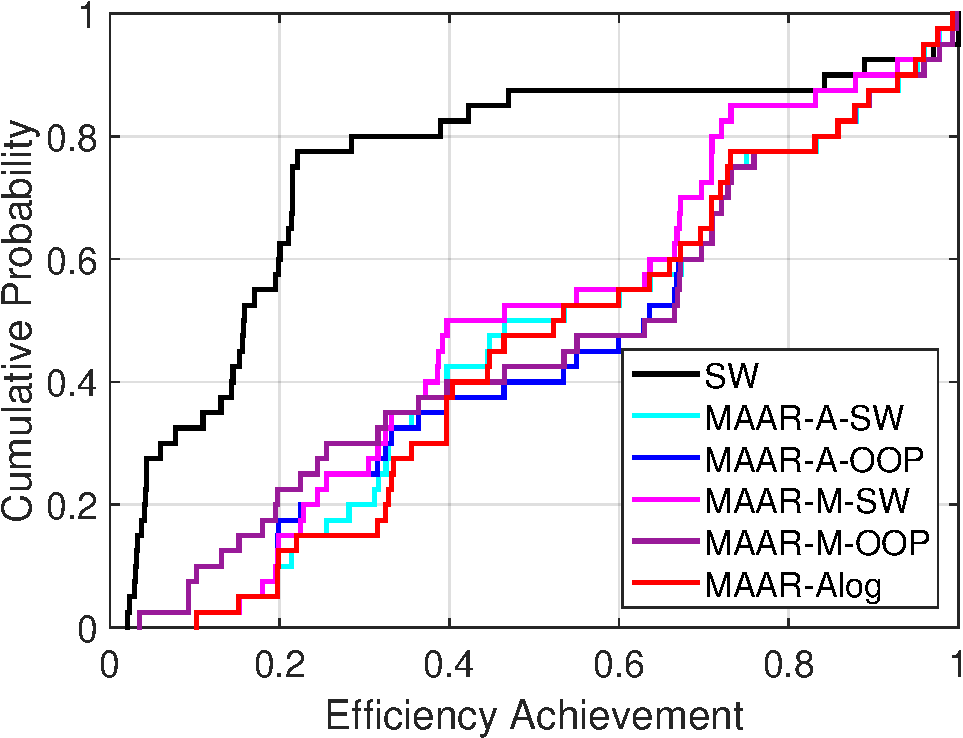
\includegraphics[width=.33\linewidth]{fig/MAARoop6.pdf}\label{fig:oop6}}
		\hfill
		\subfloat[\#ACCs=12]{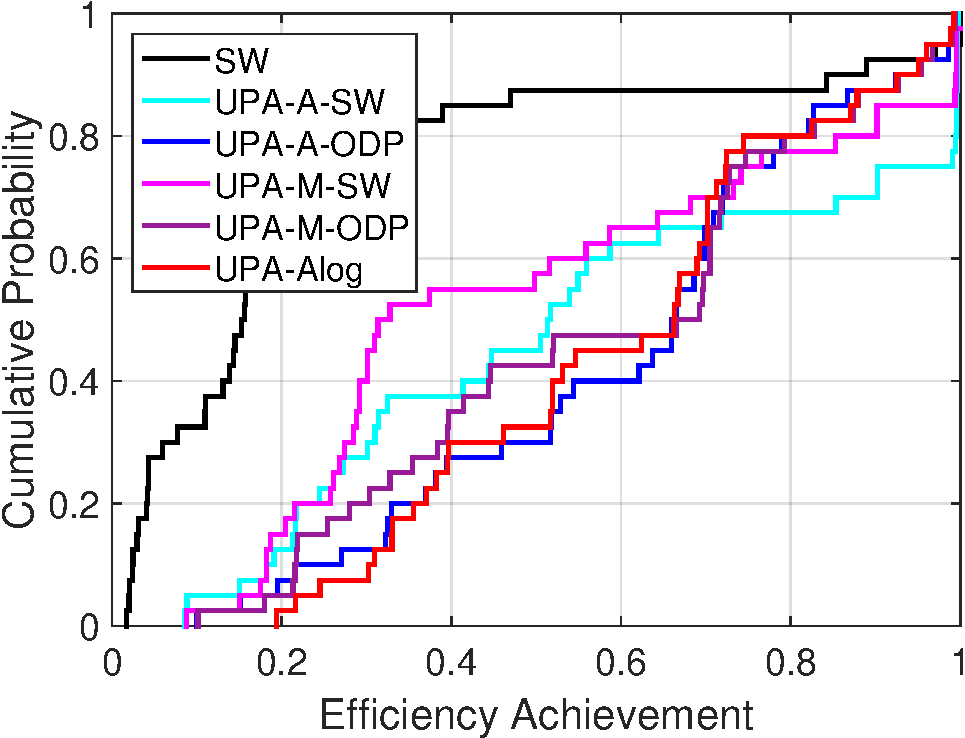
\includegraphics[width=.33\linewidth]{fig/MAARoop12.pdf}\label{fig:oop12}}
		\hfill
		\subfloat[\#ACCs=19]{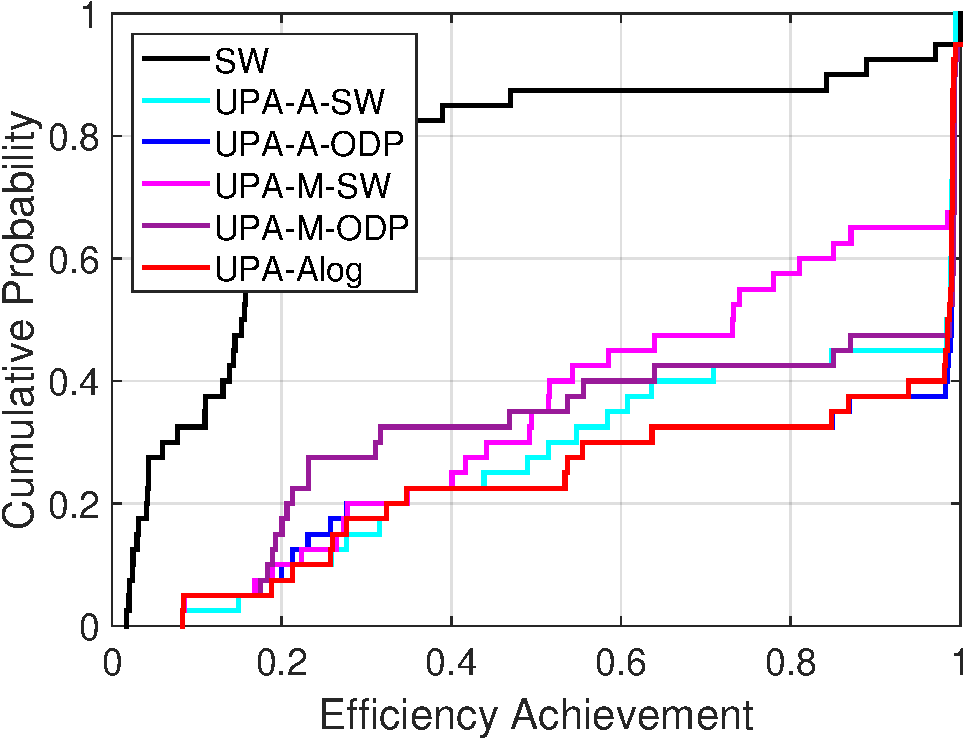
\includegraphics[width=.33\linewidth]{fig/MAARoop19.pdf}\label{fig:oop19}}
		\vspace{-8pt}
	\caption{Relative Efficiency Compared with ODP}
	\label{fig:OpenVXoop}
%		\vspace{-0pt}
\end{figure*}


Similarly, \figref{fig:OpenVXoop} displays cumulative probability of efficiency achievement ($rEFF_{ODP}$) for different aggregations in UPA with different HW budgets. The SW lines (black) are the lower bounds of efficiency achievement in these figures. 
From ACCs=6 (\figref{fig:oop6}) to ACCs=19 (\figref{fig:oop19}), UPA lines move toward the bottom right, which means they approach an overall higher efficiency achievement for applications. Comparing different aggregations in UPA, $A\mhyphen SW$ is also good for high-efficiency applications but loses for median- and low-efficiency applications. 
$M\mhyphen SW$ and $M\mhyphen ODP$ have big efficiency losses in \figref{fig:oop12} and \figref{fig:oop19}. 
%Like in the efficiency improvement view, $A\mhyphen OOP$ and $Alog$ achieve good performance for all applications in the achievement view.
$A\mhyphen ODP$ and $Alog$ both achieve good efficiency across all applications, but $Alog$ slightly favors lower performing applications. 
%We select $Alog$ as aggregation, since it is more fair to lower-performing applications. Moreover, it eliminates the need to compute the  normalization, i.e. finding the OPT platform for each application (a DSE problem in itself).